\documentclass{beamer}
\usepackage{graphicx}
\usepackage{subfig}
\usepackage{amsmath}
\usepackage{amssymb}
\usepackage{pifont}
\newcommand{\cmark}{\ding{51}}%
\newcommand{\xmark}{\ding{55}}%
\newcommand{\done}{\item[\cmark]}
\newcommand{\crossed}{\item[\xmark]}
\usepackage{xcolor}

\title{Future of Voice Agents}
\author{Christopher Hong}

\begin{document}

\frame{\titlepage}

\begin{frame}
\frametitle{Observation, Values and Mission}
\begin{itemize}
    \item The advent of large language models have enabled a new bridge between everyday people and computing
    \item AI should allow everyday people to harness the power of computation
    \item People should be in control of their computing, not vice versa
\end{itemize}
\end{frame}

\begin{frame}
\frametitle{Big Tech Voice Assistants (Alexa, Gemini, Siri)...}
\begin{itemize}
    \done Do well at some basic pre-programmed tasks
    \crossed Fail to grasp the context of voice commands
    \crossed Do not integrate well or at all with third-party applications
    \crossed Fail to transcribe words accurately that humans have no problem given a situational context (called "hot words" in speech recognition research)
\end{itemize}
\end{frame}

\begin{frame}
\frametitle{Solution}
\begin{itemize}
    \item Bridge user-intent to application-specific code using (large) language models
    \item Imbue automatic speech recognition with contextual capability for short-form transcription
    \item Give application developers the tools to contextualize voice assistance
\end{itemize}
\end{frame}

\begin{frame}
\frametitle{Prototype case: Gym Working Logging App}
\begin{columns}
\begin{column}{0.5\textwidth}
    Suppose, in a workout logging app, the user wants to switch to recording a different type (eg. "Ab Crunch Machine"). How can the user invoke a voice assistant to specify it quickly?
    \vspace{2cm}
\end{column}
\begin{column}{0.5\textwidth}
    \centering
    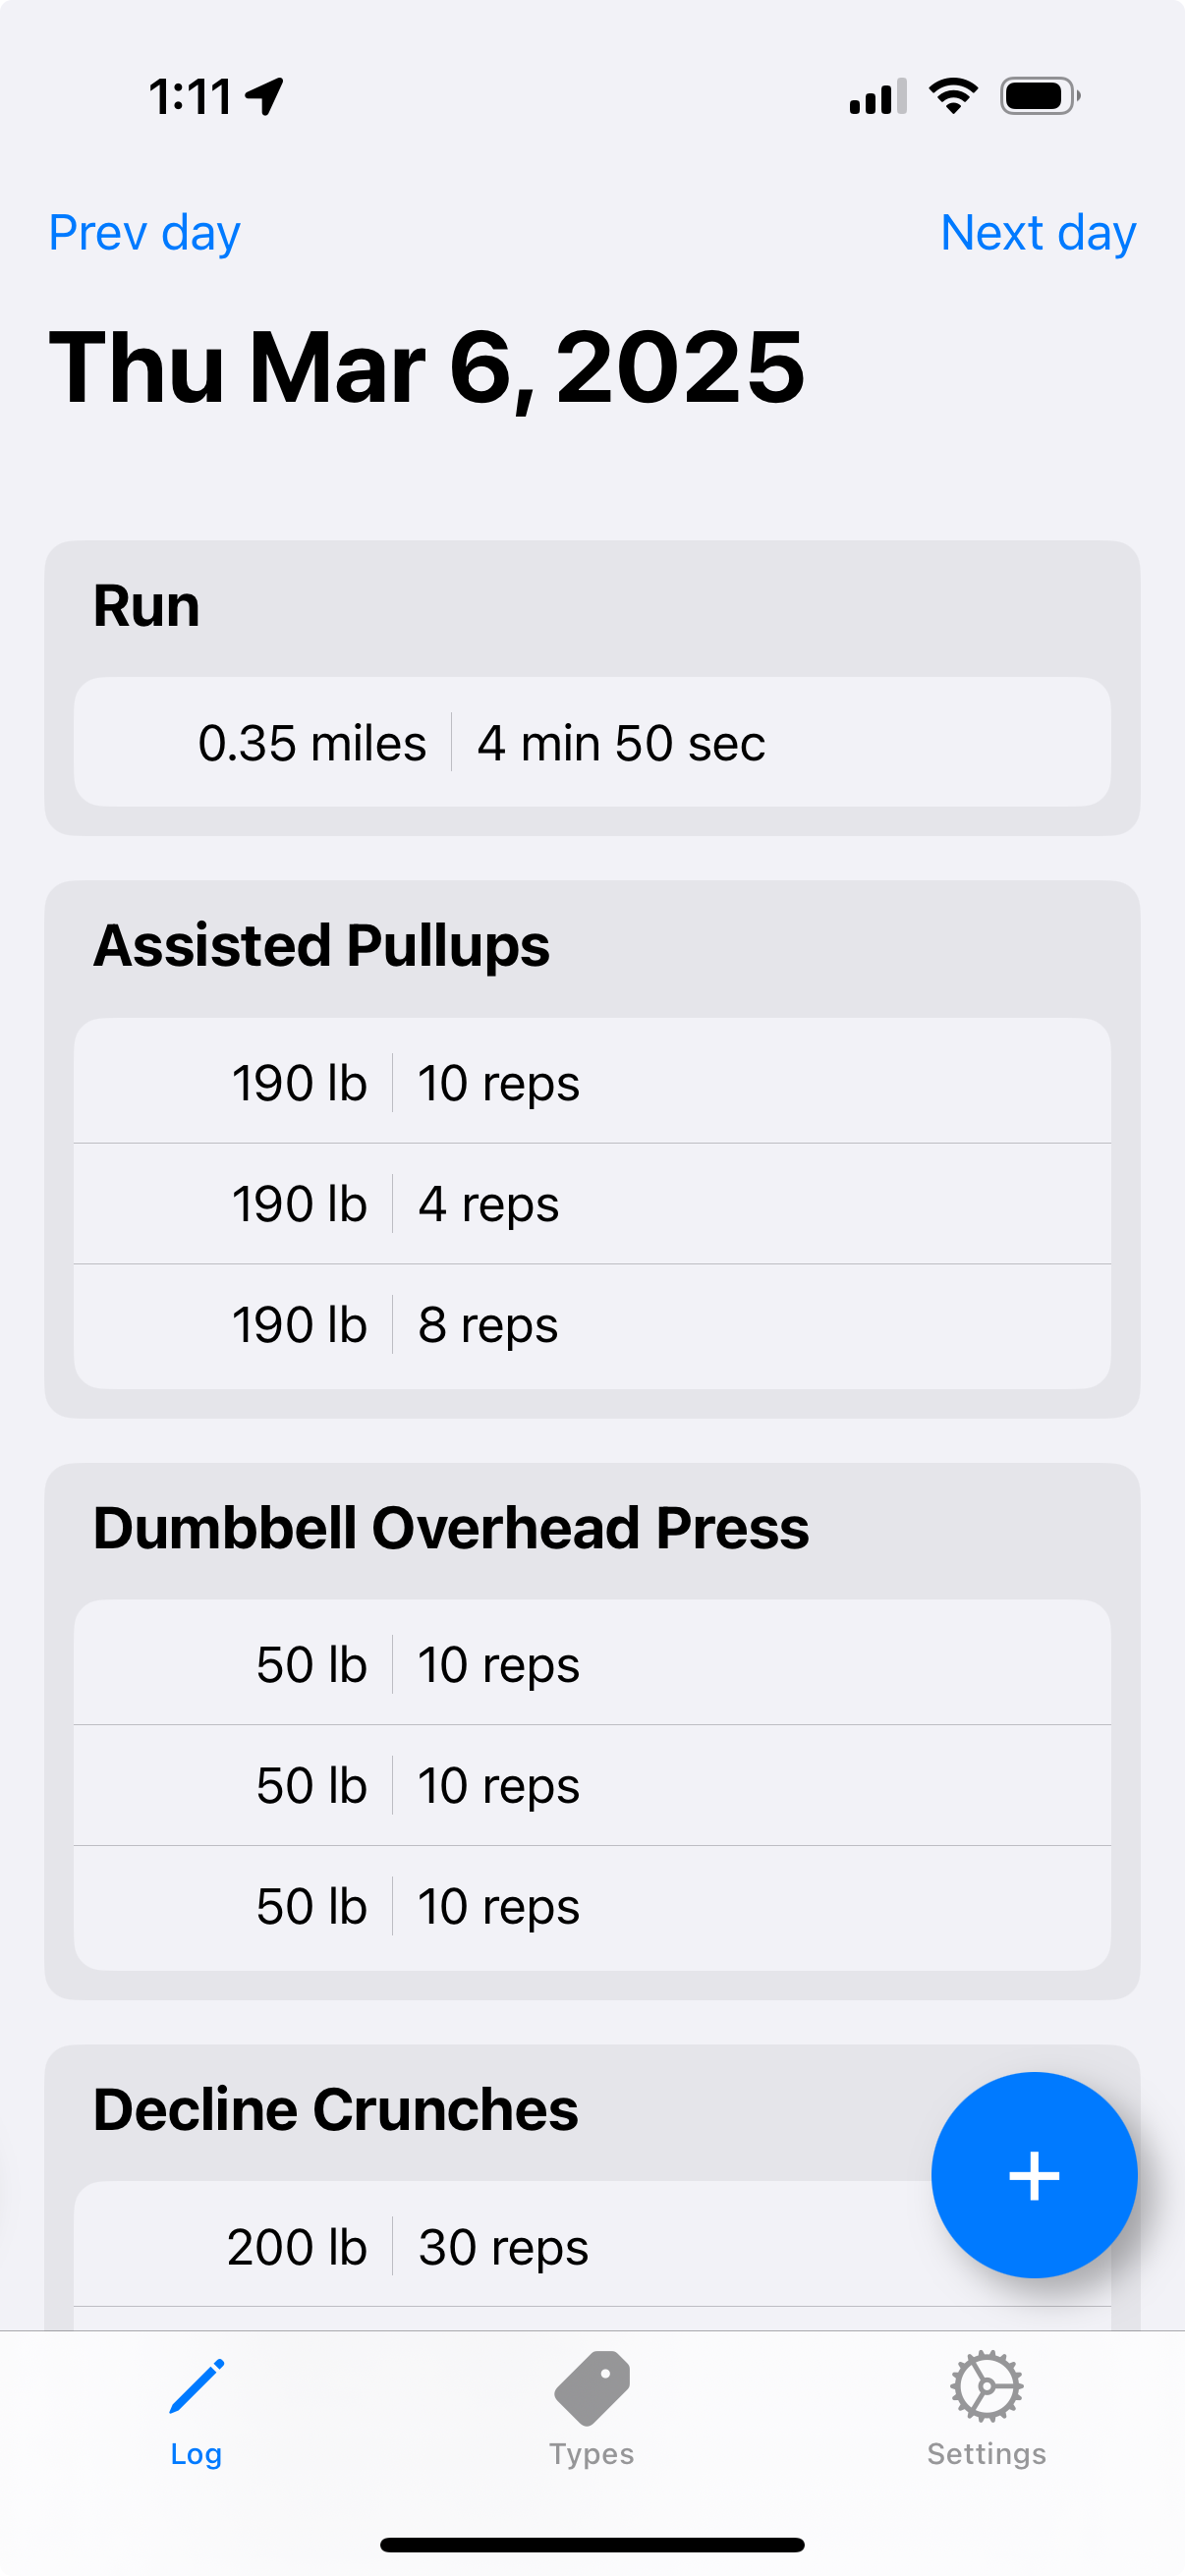
\includegraphics[height=8cm]{images/sc.png}
\end{column}
\end{columns}
\end{frame}

\begin{frame}
\frametitle{Prototype case: Gym Working Logging App}
\begin{columns}
\begin{column}{0.5\textwidth}
    Instead of using a platform or SaaS API from Apple, Google, etc., use a tailored automatic speech recognition pipeline to control quality and viability.
    \vspace{2cm}
\end{column}
\begin{column}{0.5\textwidth}
    \centering
    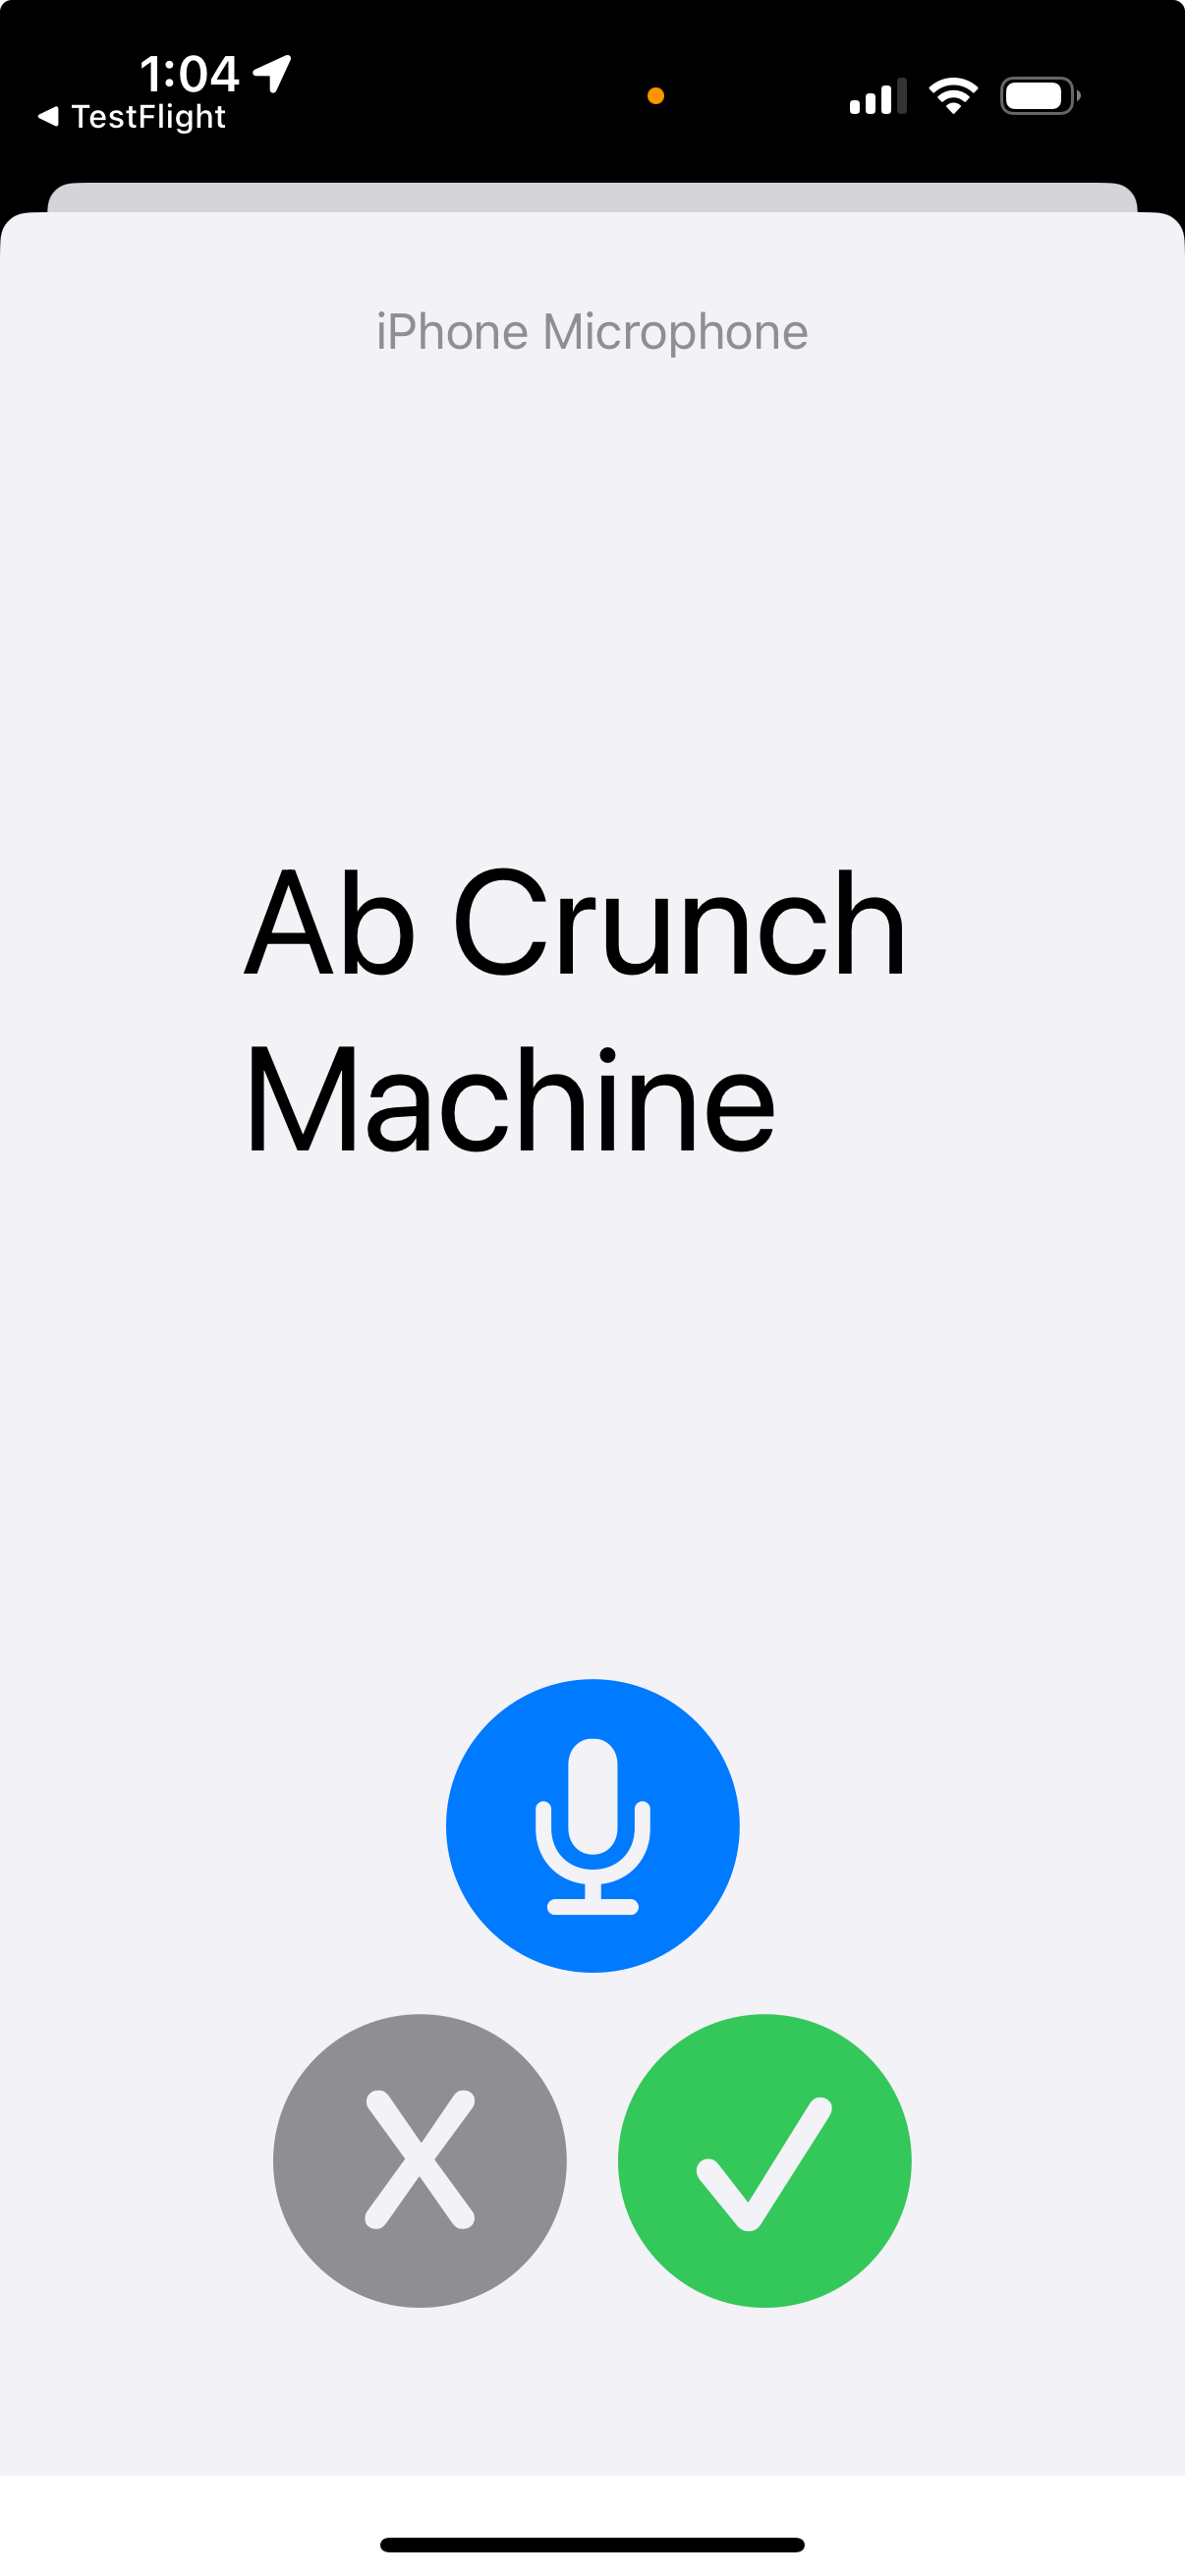
\includegraphics[height=8cm]{images/scasr.png}
\end{column}
\end{columns}
\end{frame}

\begin{frame}
\frametitle{Prototype case: Gym Working Logging App}
The app is a polished minimum-viable product that will be launched soon from the time of creating this presentation.
\end{frame}

\begin{frame}
\frametitle{Prototype case: Gym Working Logging App}
Research results below comparing "Custom" to SaaS APIs demonstrate the need for better contextualizing tools for speech recognition.
\vspace{1cm}
\centering
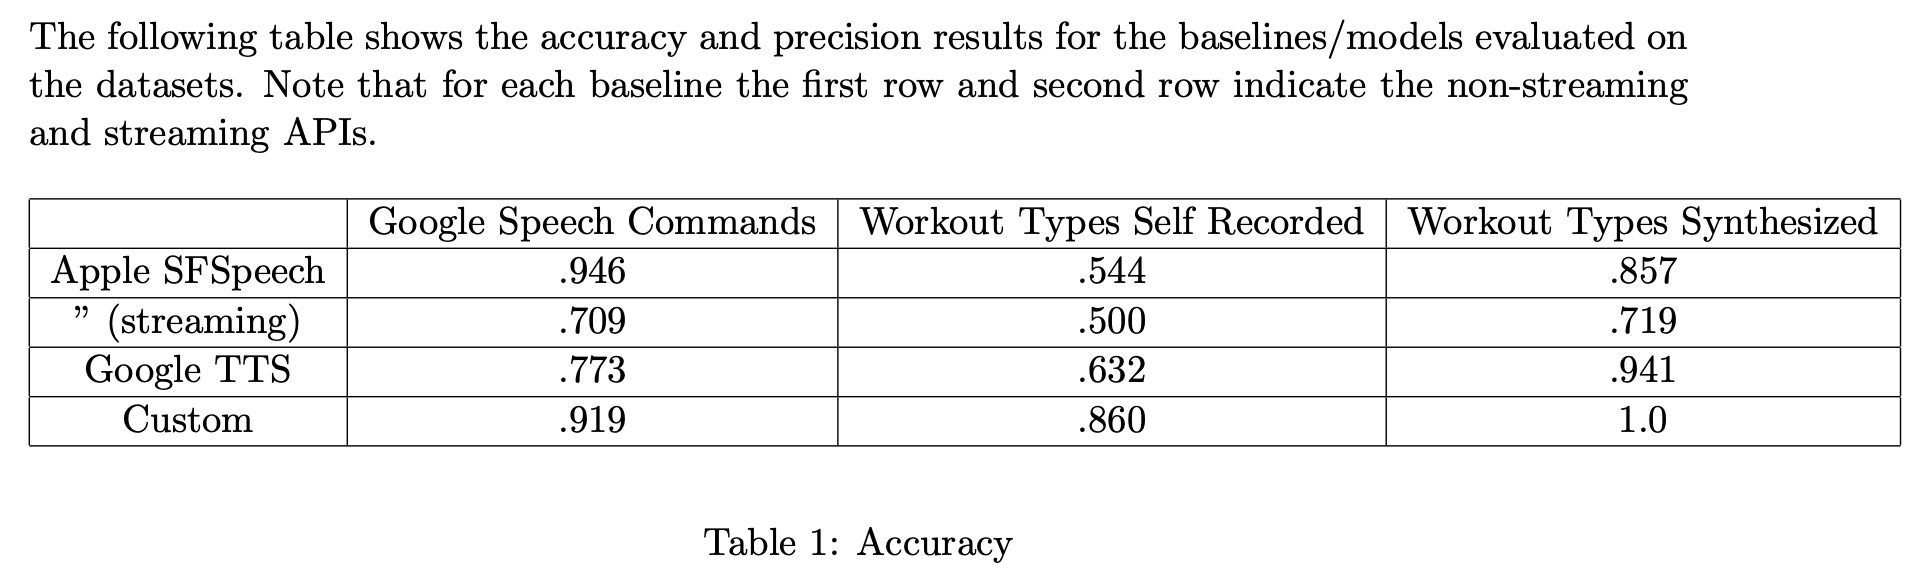
\includegraphics[height=3cm]{images/preliminary_results.png}
For a whitepaper that delves further in the technical aspects, visit 
\end{frame}

\end{document}
